% Ready-to-paste figure snippets for the diagrams in pics/ (sources: diagrams/*.puml, render with diagrams/render.sh).
% Widths are the natural size of each diagram, capped at \textwidth, so text prints at 7.5 to 9 pt.
% The comment above each figure names the outline section it was drawn for.

% Section 3.2
\begin{figure}[htbp]
	\centering
	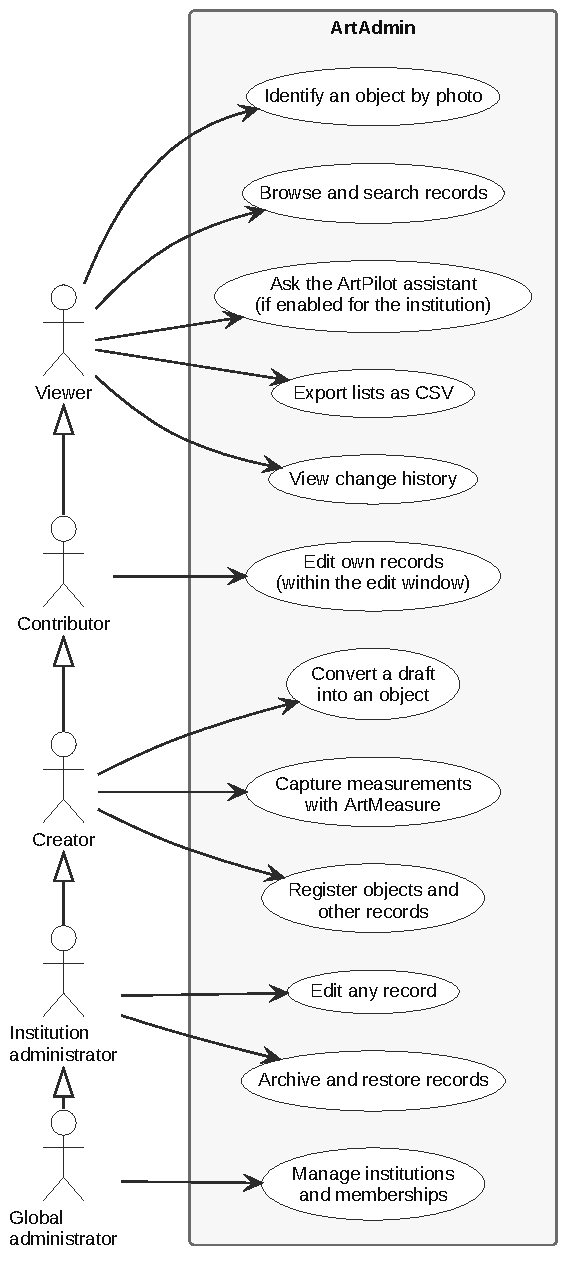
\includegraphics[width=9.8cm,height=0.86\textheight,keepaspectratio]{pics/usecase-roles.pdf}
	\caption{Use cases per membership group. Each group inherits the use cases of the group above it.}
	\label{fig:usecases}
\end{figure}

% Section 3.5
\begin{figure}[htbp]
	\centering
	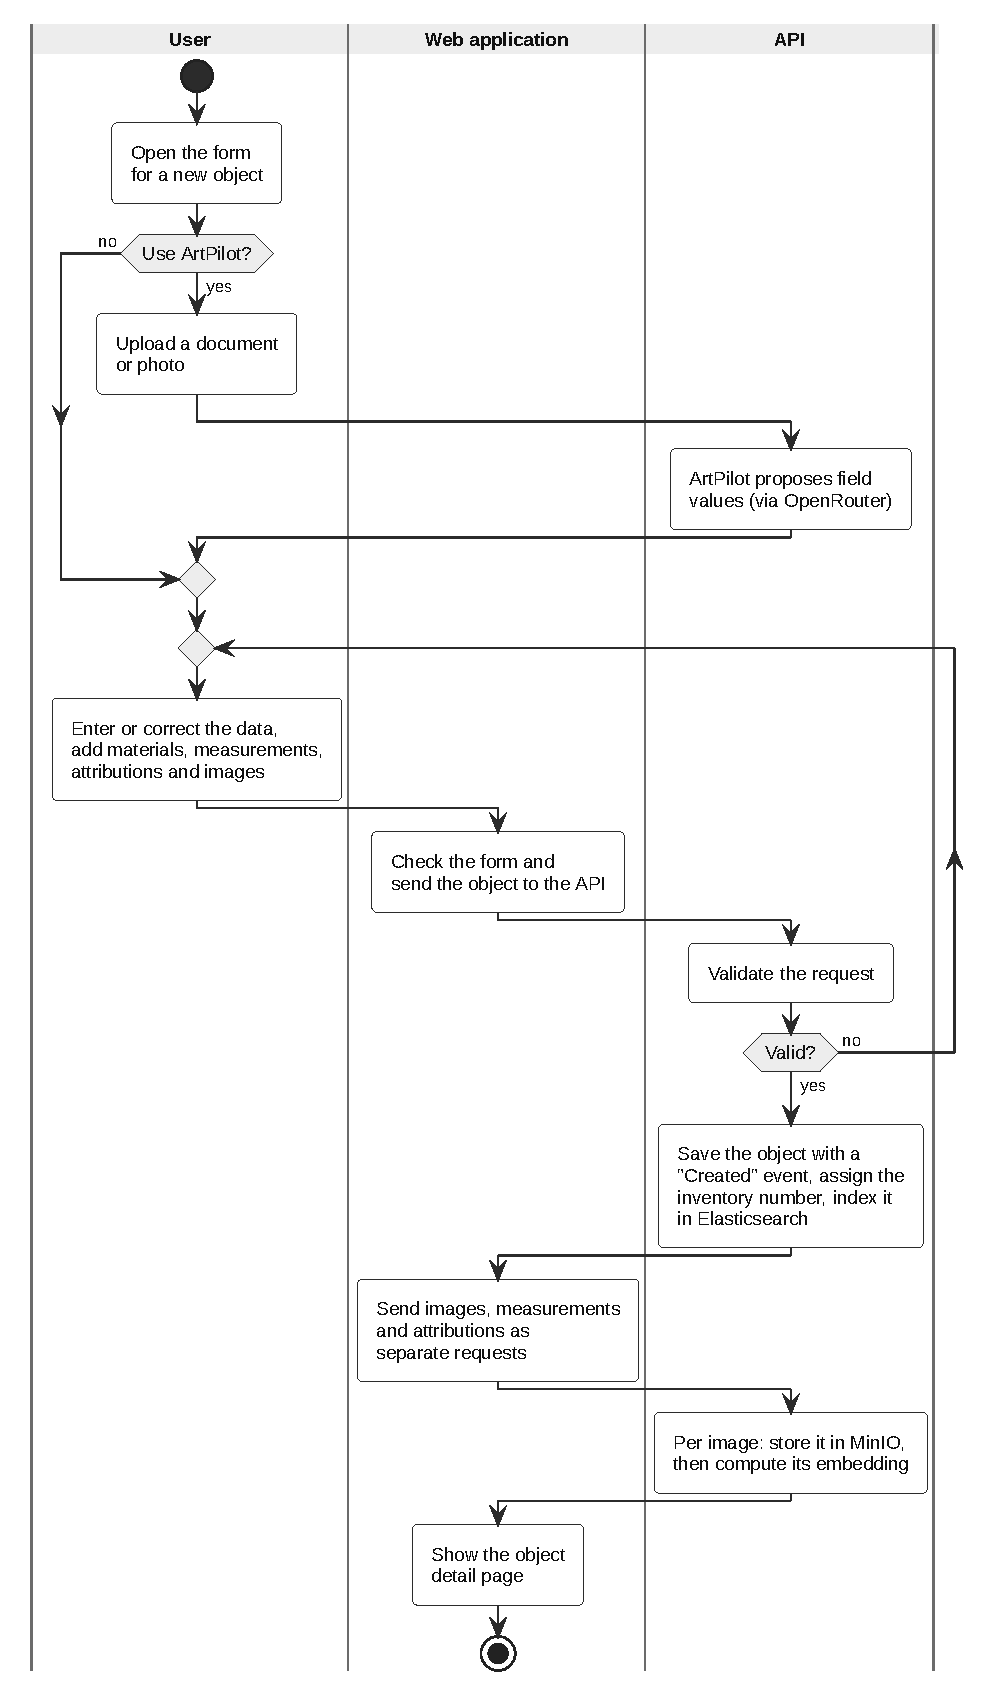
\includegraphics[width=\textwidth,height=0.86\textheight,keepaspectratio]{pics/activity-object-registration.pdf}
	\caption{Registering a new object, optionally with a proposal from ArtPilot.}
	\label{fig:activity-registration}
\end{figure}

% Section 3.5
\begin{figure}[htbp]
	\centering
	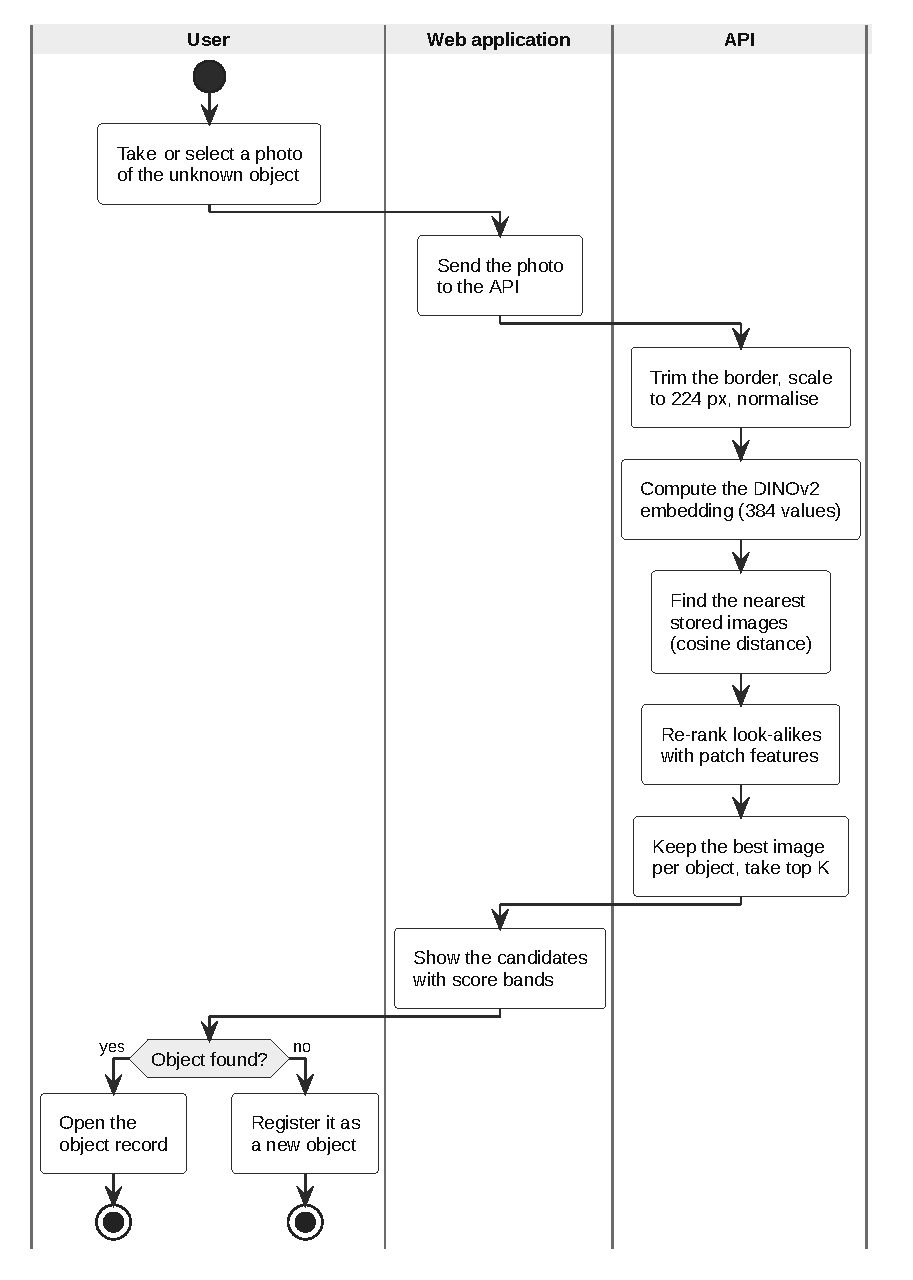
\includegraphics[width=15.5cm,height=0.86\textheight,keepaspectratio]{pics/activity-similarity-search.pdf}
	\caption{Identifying an unknown object by photo.}
	\label{fig:activity-similarity}
\end{figure}

% Section 4.1
\begin{figure}[htbp]
	\centering
	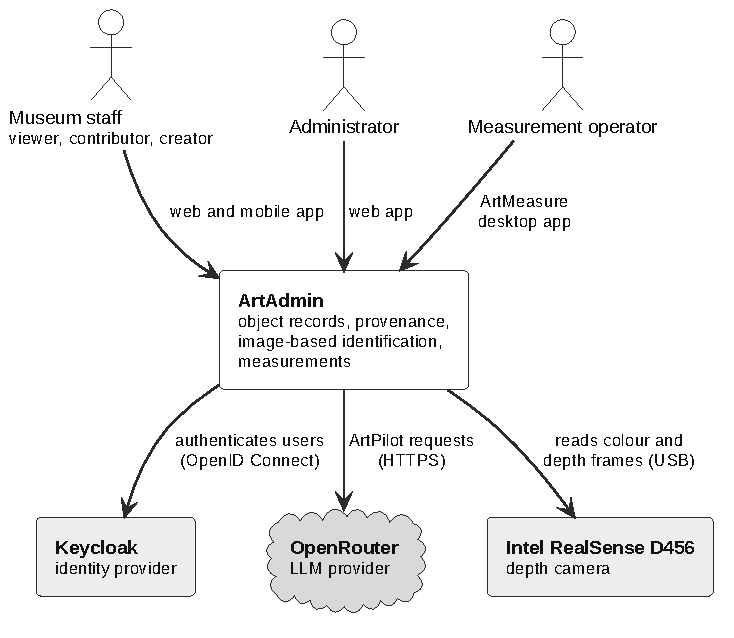
\includegraphics[width=12.4cm,height=0.86\textheight,keepaspectratio]{pics/system-context.pdf}
	\caption{System context of ArtAdmin with its users and external systems.}
	\label{fig:system-context}
\end{figure}

% Section 4.1
\begin{figure}[htbp]
	\centering
	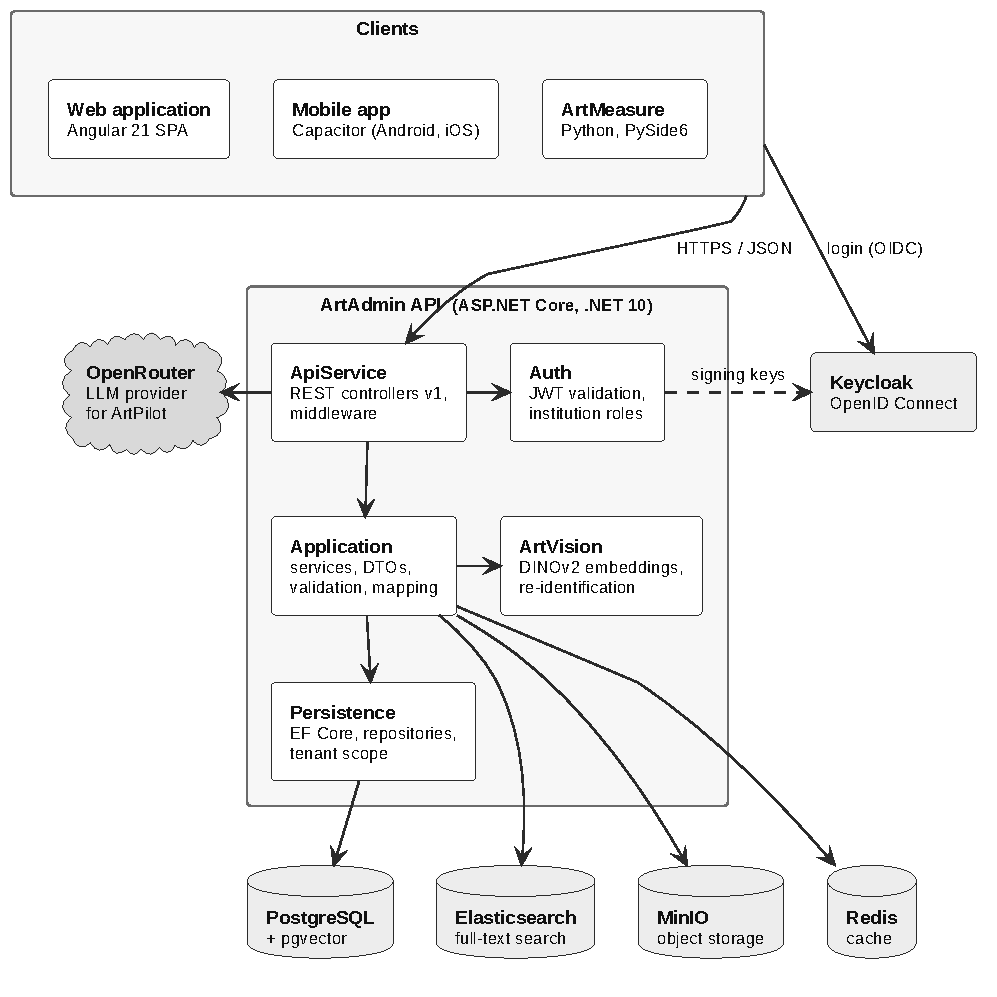
\includegraphics[width=\textwidth,height=0.86\textheight,keepaspectratio]{pics/component-overview.pdf}
	\caption{Components of ArtAdmin and the services they depend on.}
	\label{fig:components}
\end{figure}

% Section 4.1
\begin{figure}[htbp]
	\centering
	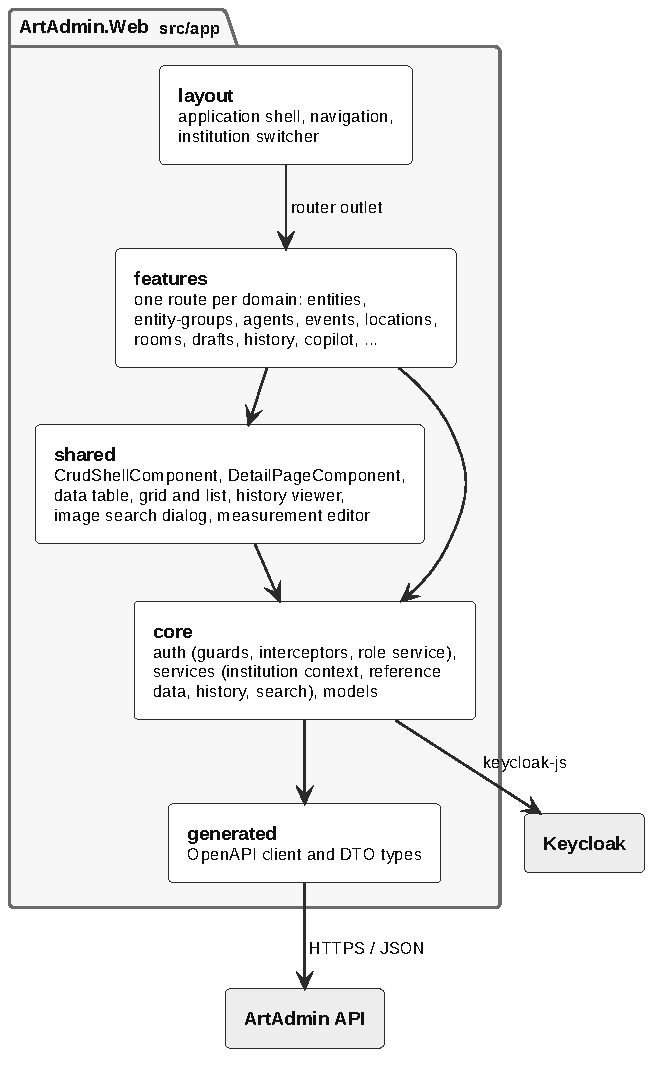
\includegraphics[width=11.3cm,height=0.86\textheight,keepaspectratio]{pics/frontend-structure.pdf}
	\caption{Structure of the Angular web application.}
	\label{fig:frontend-structure}
\end{figure}

% Section 4.2
\begin{figure}[htbp]
	\centering
	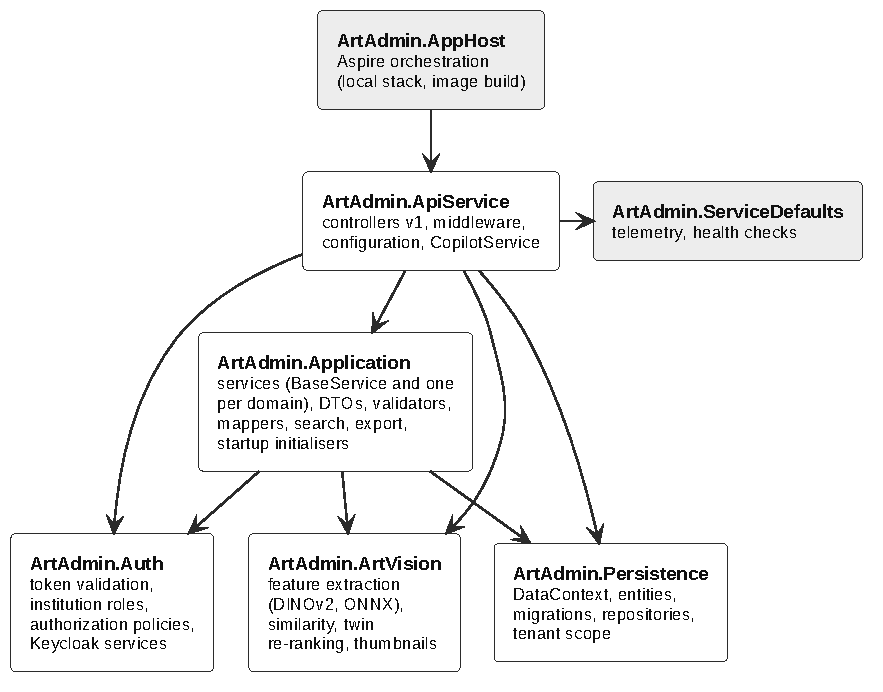
\includegraphics[width=15.0cm,height=0.86\textheight,keepaspectratio]{pics/backend-layers.pdf}
	\caption{Projects of the backend solution and their references.}
	\label{fig:backend-layers}
\end{figure}

% Section 4.2
\begin{figure}[htbp]
	\centering
	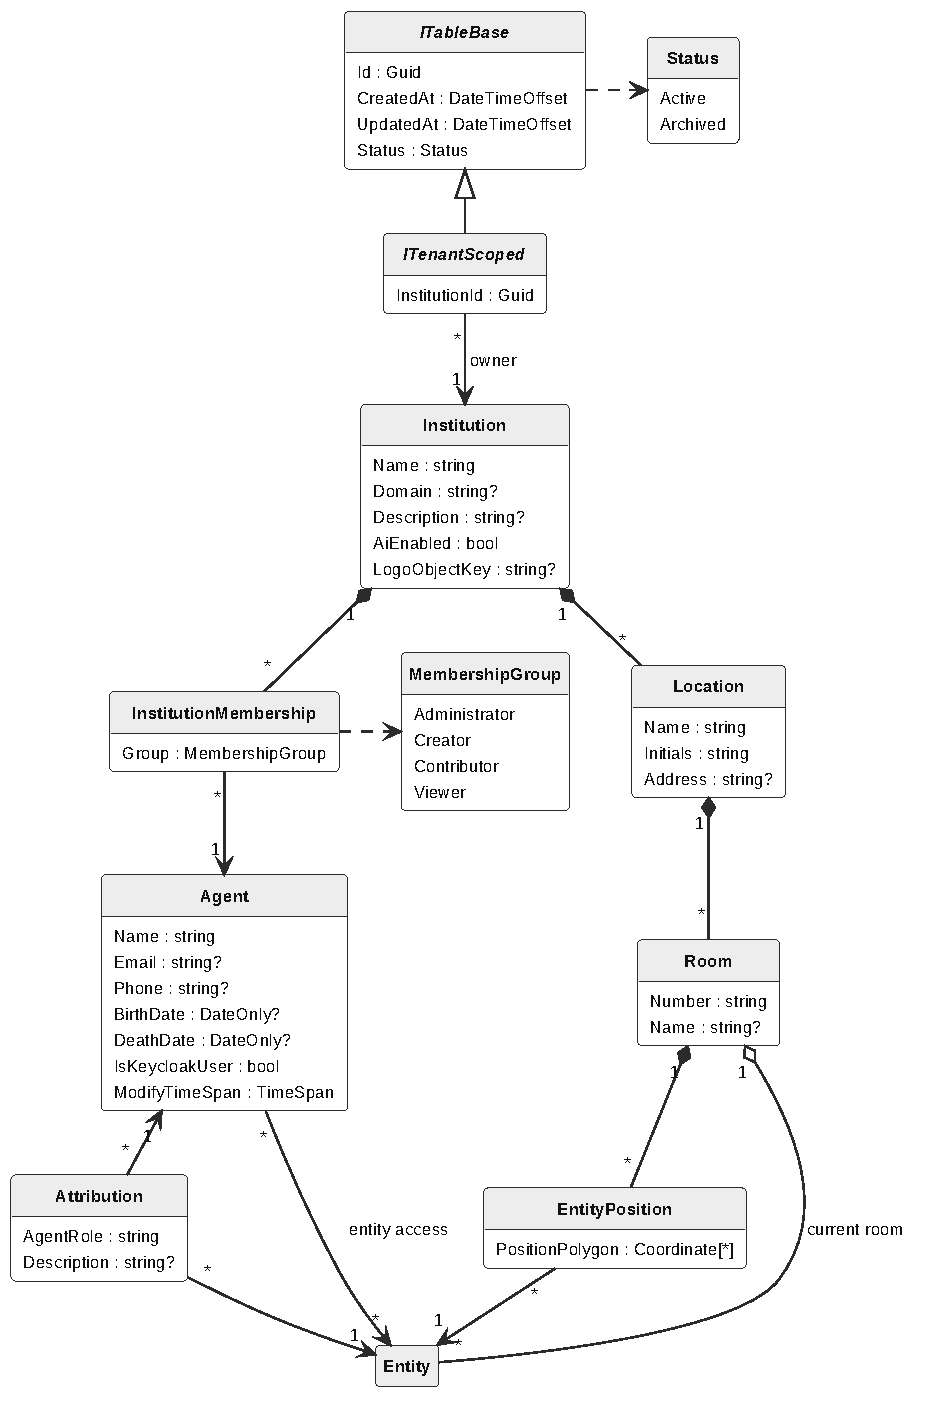
\includegraphics[width=\textwidth,height=0.86\textheight,keepaspectratio]{pics/class-tenancy-agents.pdf}
	\caption{Domain model: base types, institutions, memberships, agents and locations. Grey classes are detailed in another figure.}
	\label{fig:class-tenancy}
\end{figure}

% Section 4.2
\begin{figure}[htbp]
	\centering
	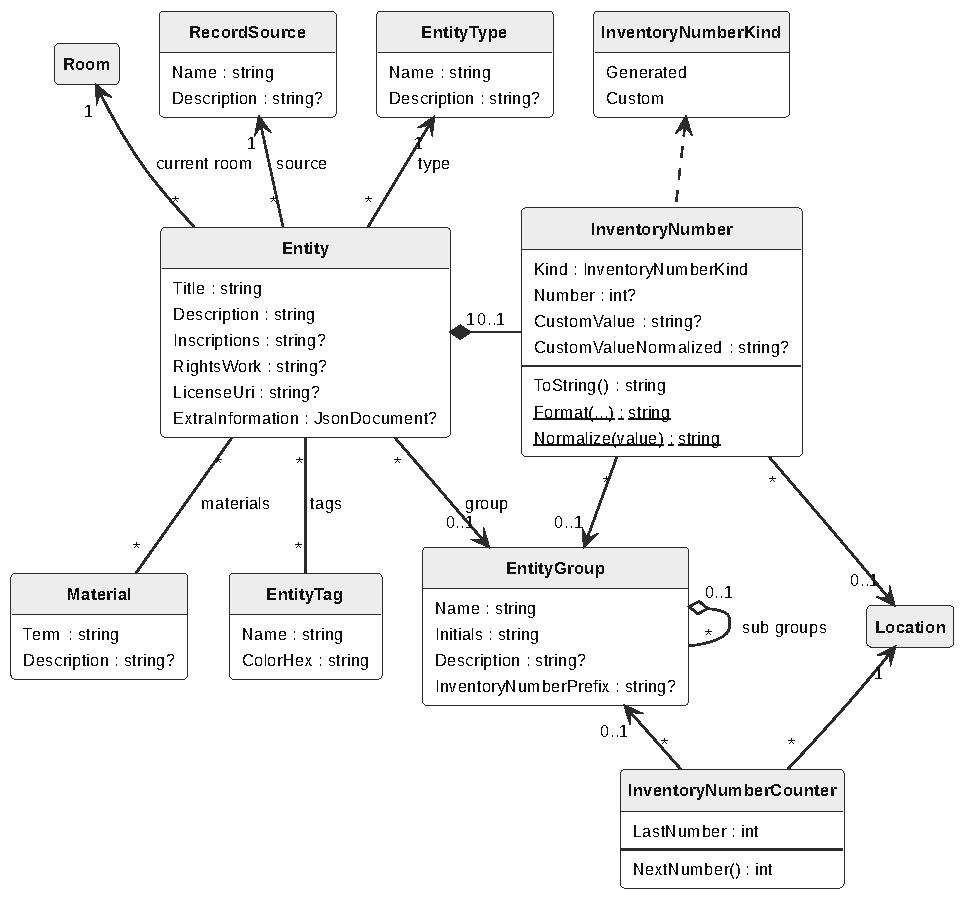
\includegraphics[width=\textwidth,height=0.86\textheight,keepaspectratio]{pics/class-objects.pdf}
	\caption{Domain model: objects, groups, reference data and inventory numbers. Grey classes are detailed in another figure.}
	\label{fig:class-objects}
\end{figure}

% Section 4.2
\begin{figure}[htbp]
	\centering
	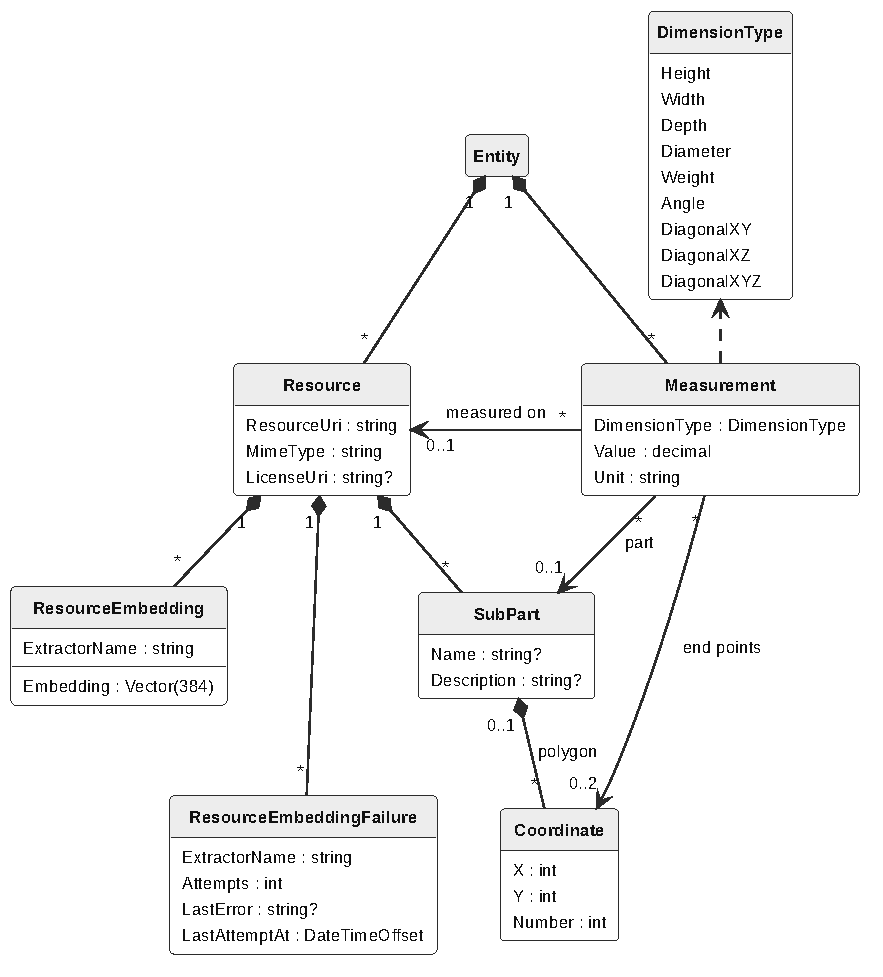
\includegraphics[width=14.9cm,height=0.86\textheight,keepaspectratio]{pics/class-media-measurements.pdf}
	\caption{Domain model: images, embeddings, sub-parts and measurements. Grey classes are detailed in another figure.}
	\label{fig:class-media}
\end{figure}

% Section 4.2
\begin{figure}[htbp]
	\centering
	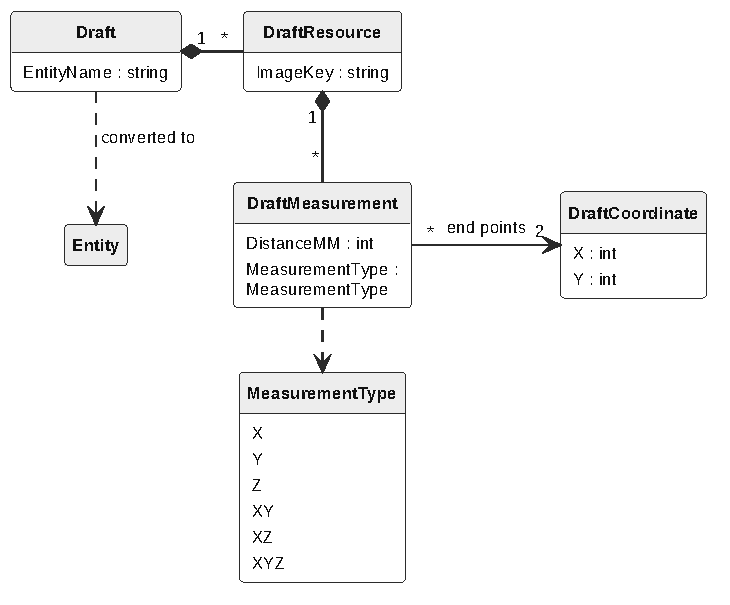
\includegraphics[width=12.4cm,height=0.86\textheight,keepaspectratio]{pics/class-drafts.pdf}
	\caption{Domain model: measurement drafts uploaded by ArtMeasure.}
	\label{fig:class-drafts}
\end{figure}

% Section 4.2
\begin{figure}[htbp]
	\centering
	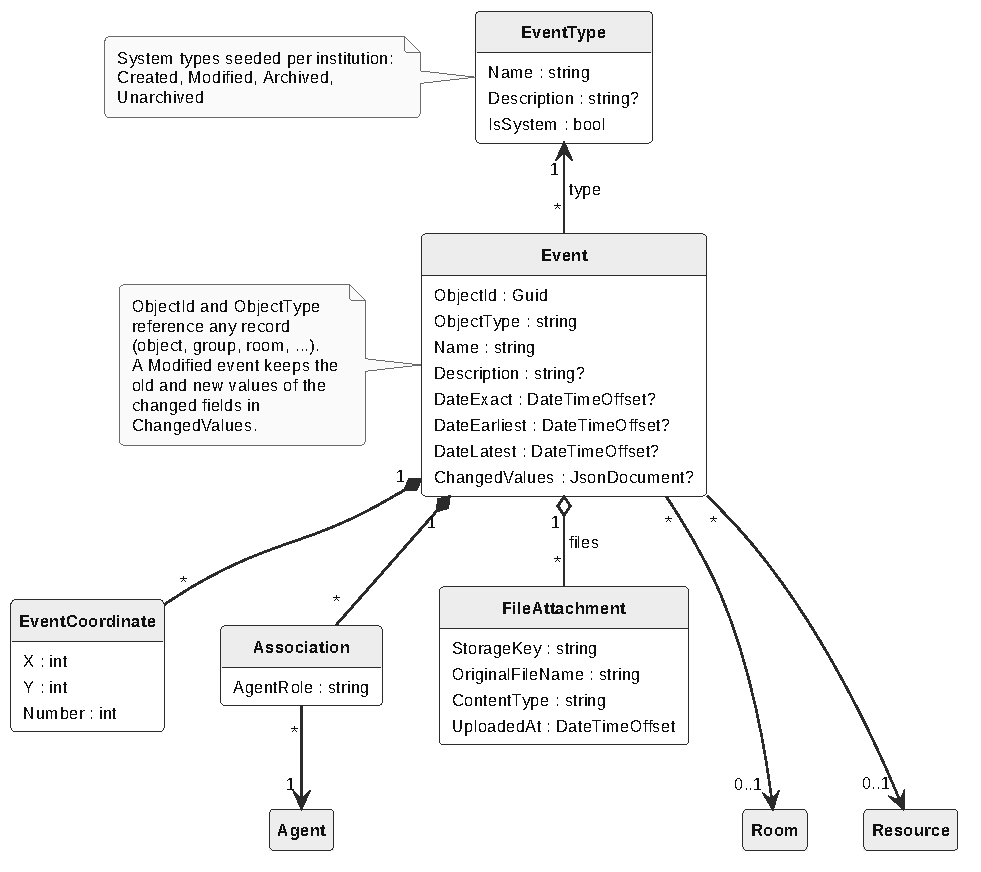
\includegraphics[width=\textwidth,height=0.86\textheight,keepaspectratio]{pics/class-history.pdf}
	\caption{Domain model: events, associations and file attachments. Grey classes are detailed in another figure.}
	\label{fig:class-history}
\end{figure}

% Section 4.2
\begin{figure}[htbp]
	\centering
	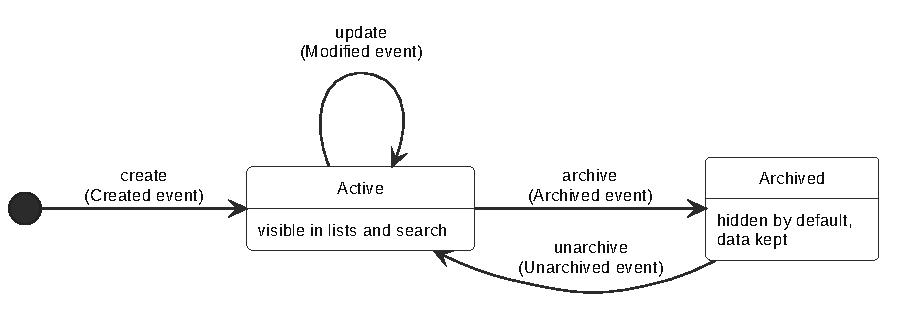
\includegraphics[width=15.3cm,height=0.86\textheight,keepaspectratio]{pics/state-record-lifecycle.pdf}
	\caption{Life cycle of a record. Records are archived instead of deleted.}
	\label{fig:record-lifecycle}
\end{figure}

% Section 4.4
\begin{figure}[htbp]
	\centering
	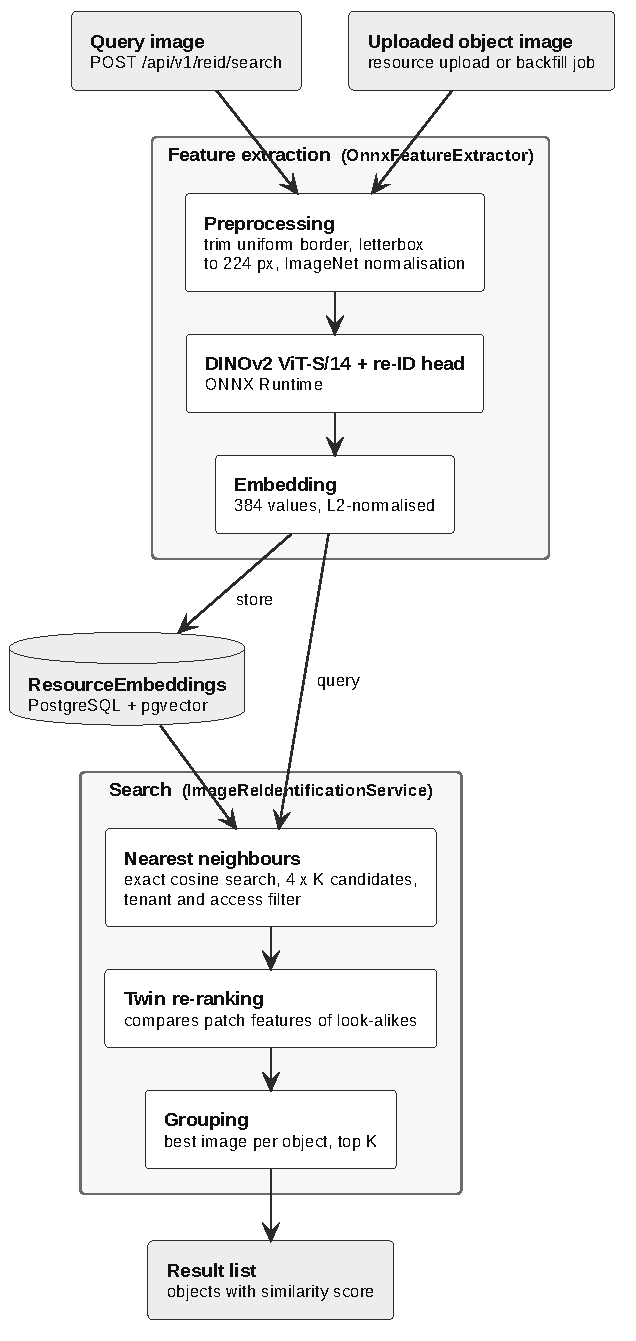
\includegraphics[width=10.8cm,height=0.86\textheight,keepaspectratio]{pics/reid-pipeline.pdf}
	\caption{Image re-identification pipeline from image to result list.}
	\label{fig:reid-pipeline}
\end{figure}

% Section 4.5
\begin{figure}[htbp]
	\centering
	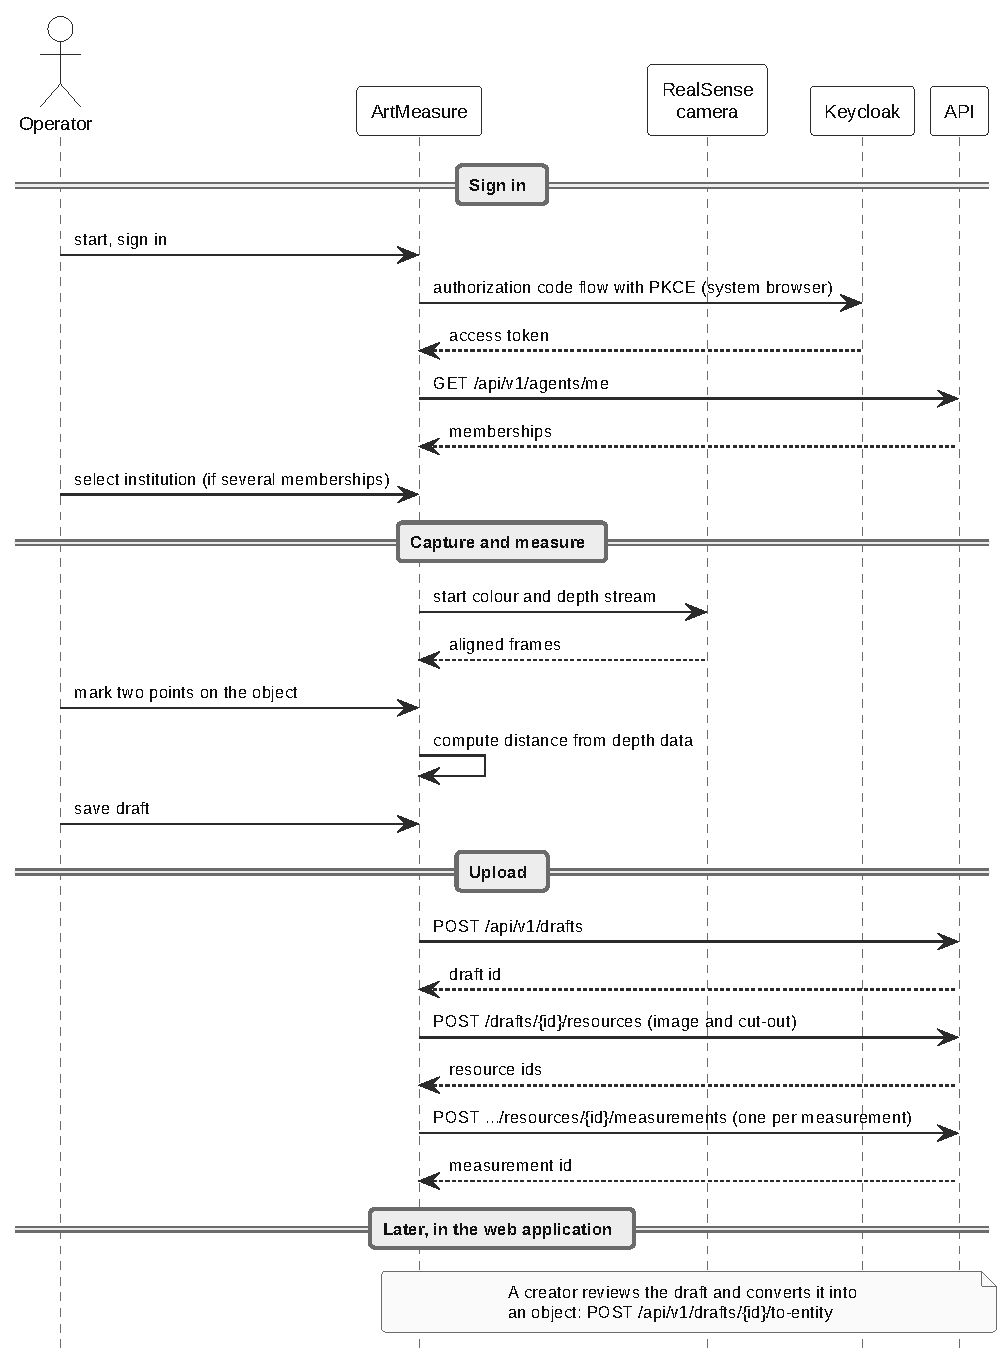
\includegraphics[width=\textwidth,height=0.86\textheight,keepaspectratio]{pics/seq-artmeasure-draft.pdf}
	\caption{ArtMeasure: sign-in, capture, measurement and upload of a draft.}
	\label{fig:seq-artmeasure}
\end{figure}

% Section 4.6
\begin{figure}[htbp]
	\centering
	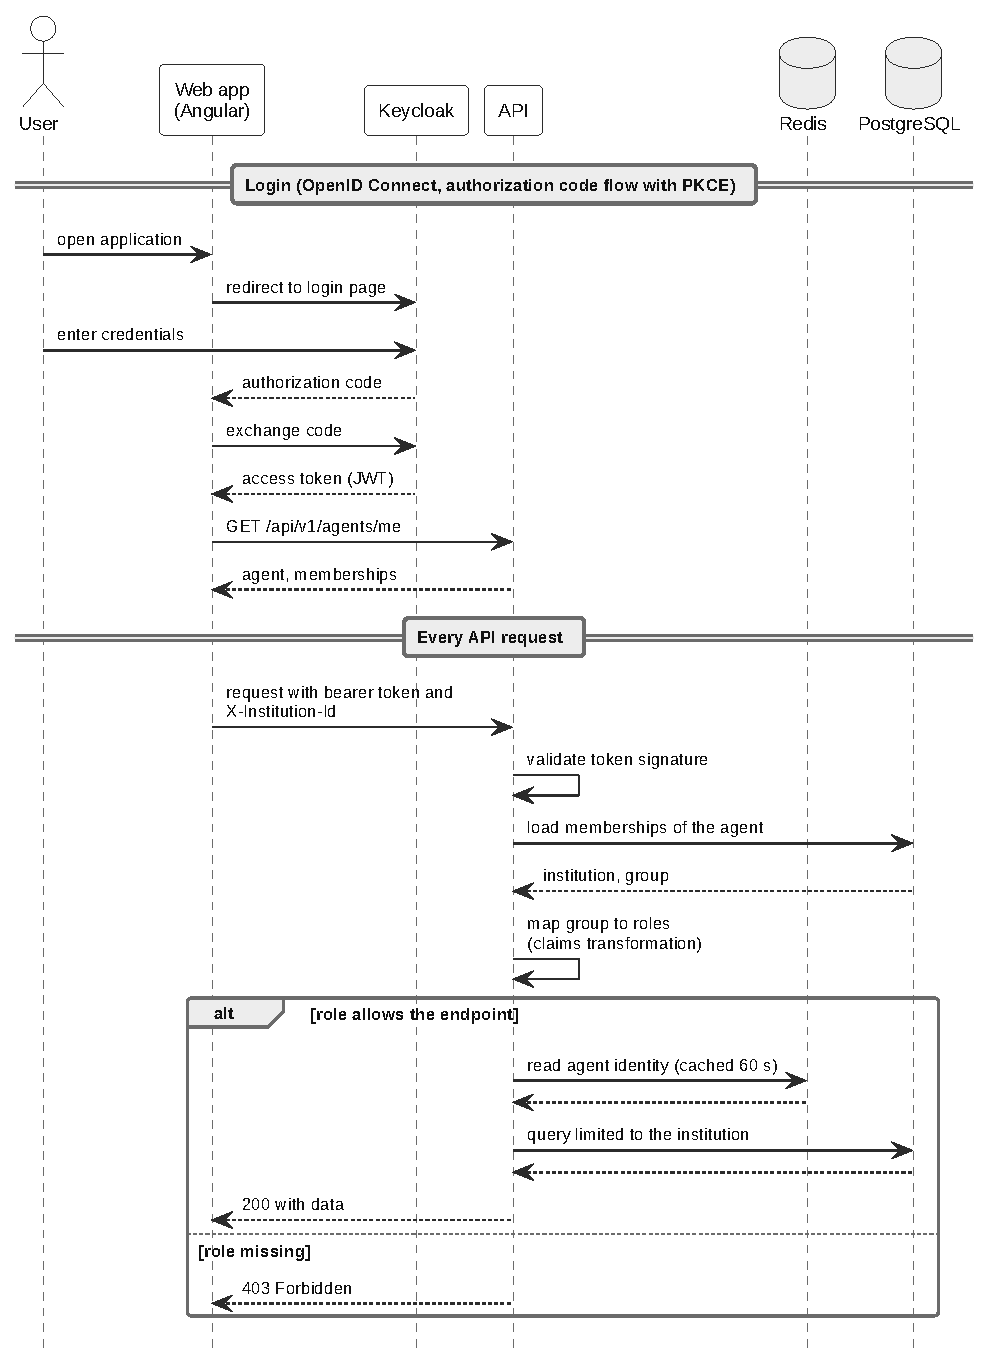
\includegraphics[width=\textwidth,height=0.86\textheight,keepaspectratio]{pics/seq-auth-request.pdf}
	\caption{Login with Keycloak and resolution of institution roles on every API request.}
	\label{fig:seq-auth}
\end{figure}

% Section 4.7
\begin{figure}[htbp]
	\centering
	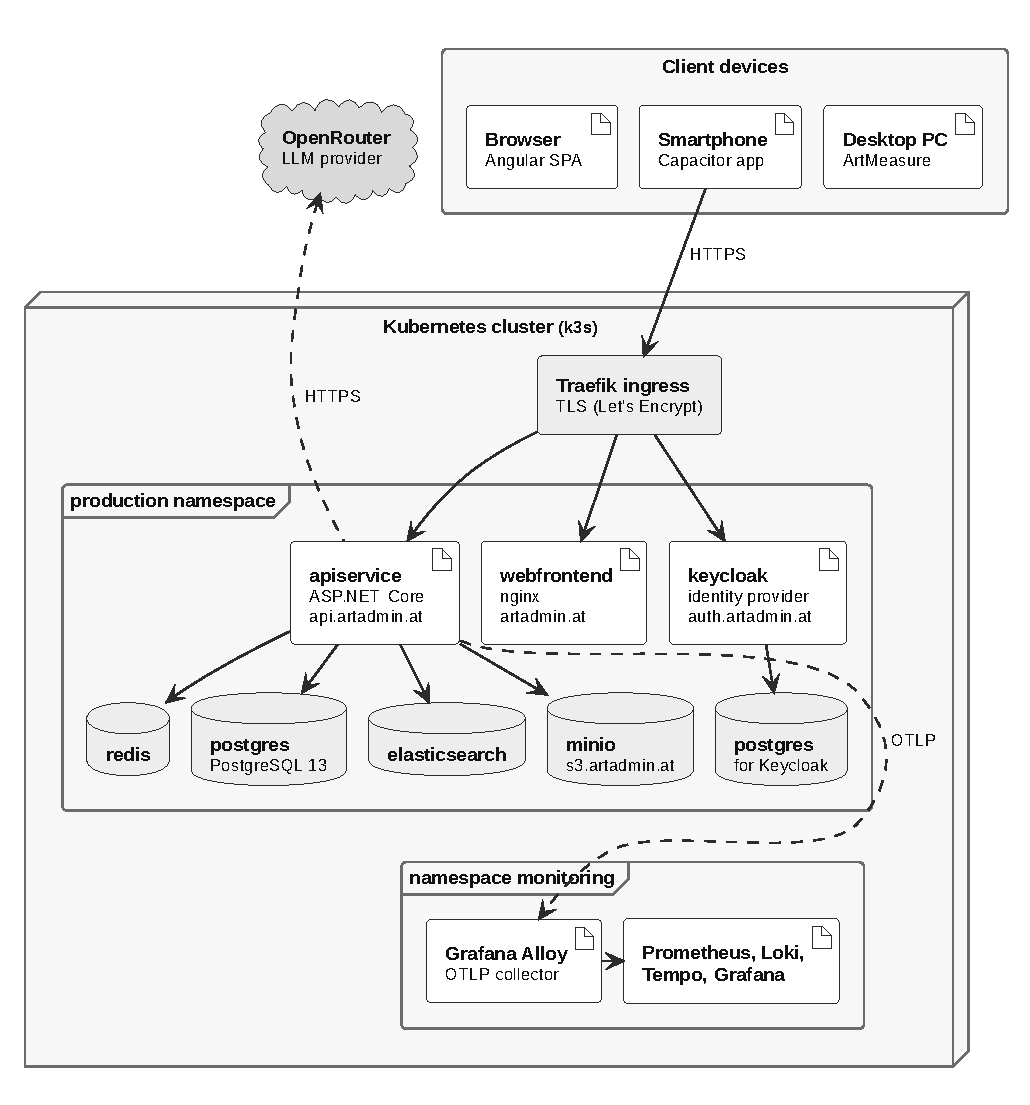
\includegraphics[width=\textwidth,height=0.86\textheight,keepaspectratio]{pics/deployment-production.pdf}
	\caption{Production deployment on the Kubernetes cluster (target manifests). The image search needs the pgvector extension, which the PostgreSQL 13 instance does not provide yet.}
	\label{fig:deployment-production}
\end{figure}

% Section 4.7
\begin{figure}[htbp]
	\centering
	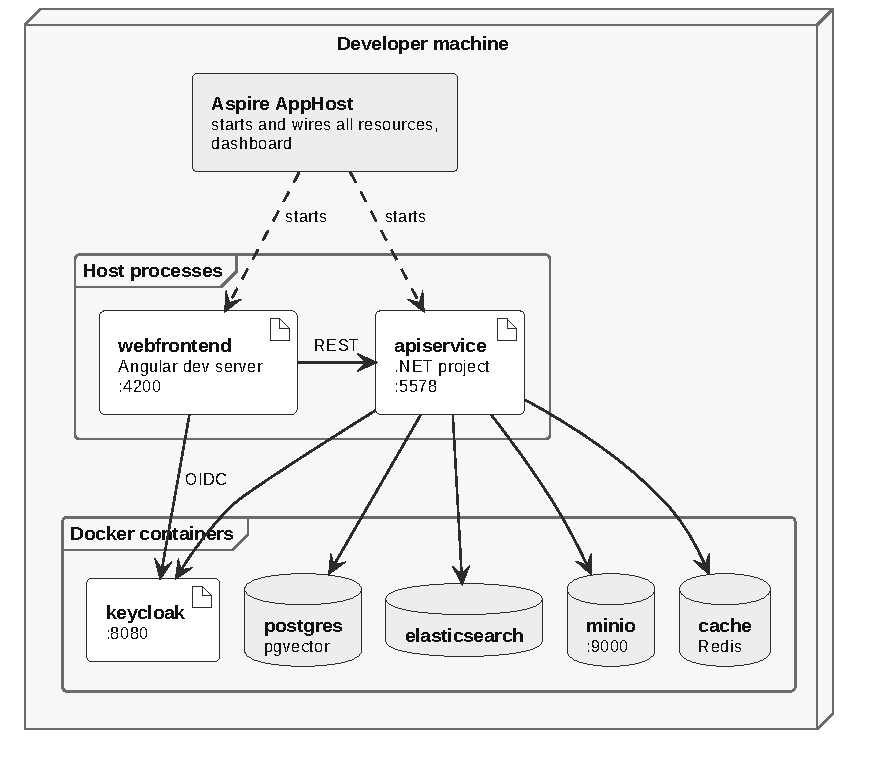
\includegraphics[width=14.8cm,height=0.86\textheight,keepaspectratio]{pics/deployment-local-aspire.pdf}
	\caption{Local development environment started by the Aspire AppHost.}
	\label{fig:deployment-local}
\end{figure}

% Section 4.7
\begin{figure}[htbp]
	\centering
	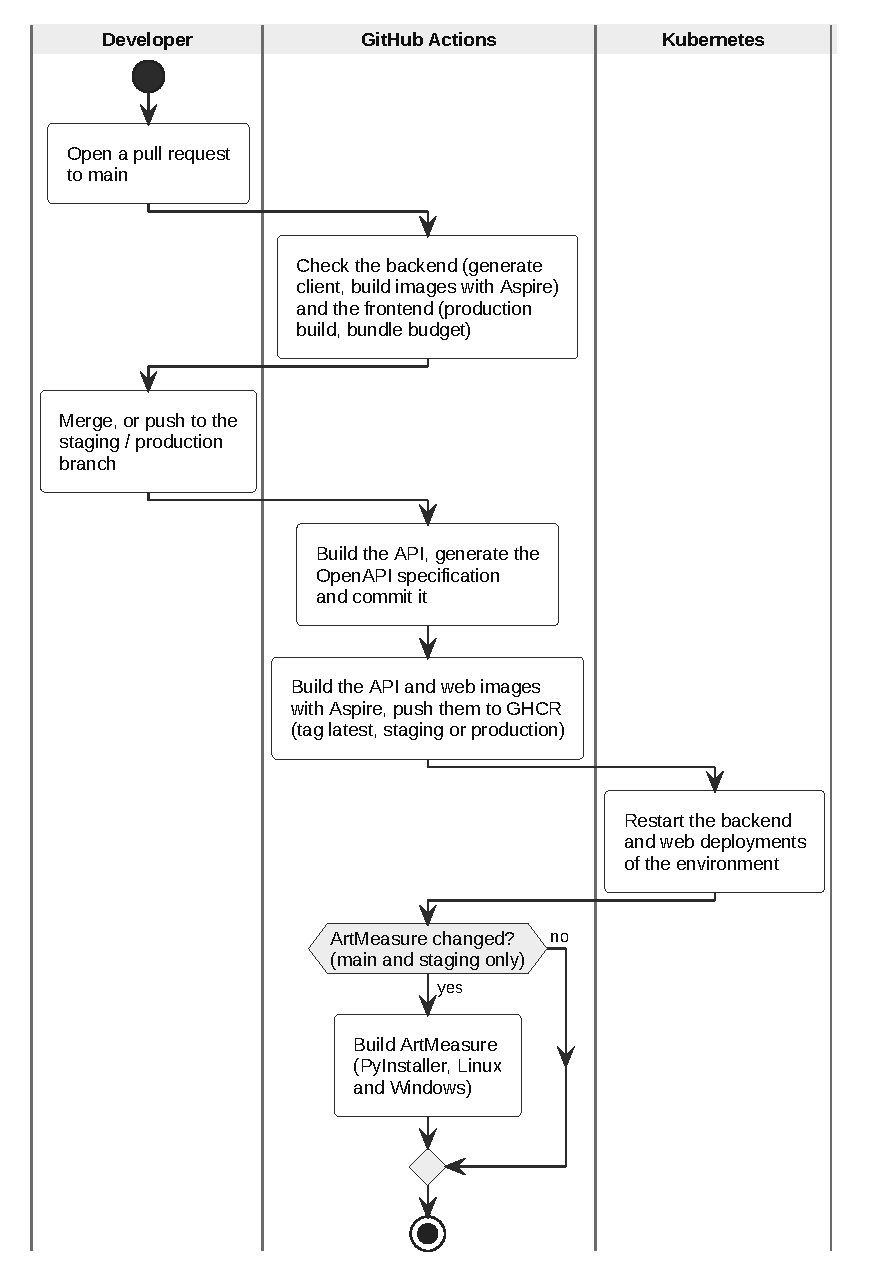
\includegraphics[width=14.7cm,height=0.86\textheight,keepaspectratio]{pics/cicd-pipeline.pdf}
	\caption{Build and deployment pipeline with GitHub Actions. The mobile apps are built by a separate workflow that runs in parallel.}
	\label{fig:cicd}
\end{figure}

% Section Appendix B
\begin{figure}[htbp]
	\centering
	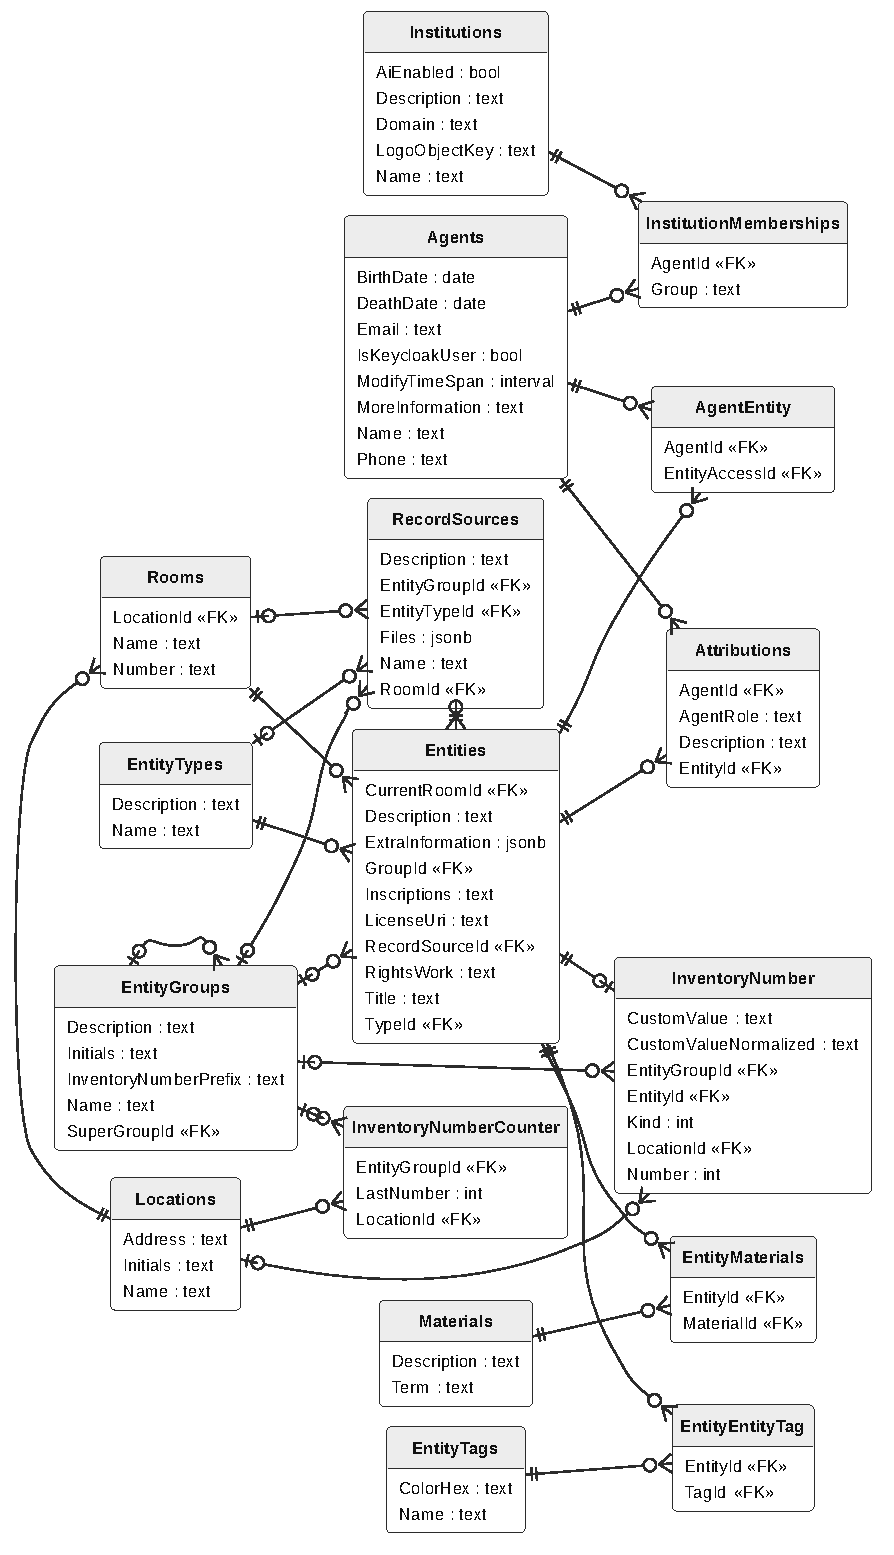
\includegraphics[width=15.1cm,height=0.86\textheight,keepaspectratio]{pics/er-core.pdf}
	\caption{Database schema, part 1: institutions, agents, locations, objects and reference data. Every table also has the columns Id, CreatedAt, UpdatedAt and Status; all tables except Agents, Institutions and the pure join tables also have InstitutionId. Grey tables are detailed in another part.}
	\label{fig:er-core}
\end{figure}

% Section Appendix B
\begin{figure}[htbp]
	\centering
	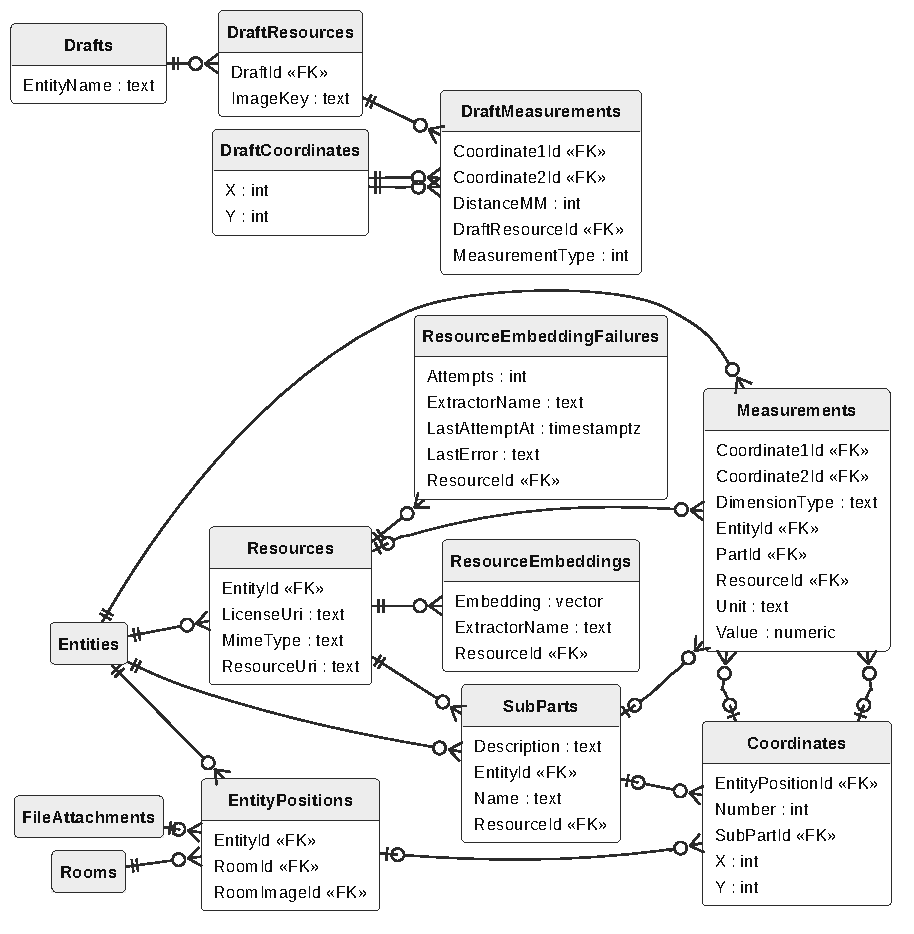
\includegraphics[width=15.5cm,height=0.86\textheight,keepaspectratio]{pics/er-media-drafts.pdf}
	\caption{Database schema, part 2: images, embeddings, measurements, positions and drafts.}
	\label{fig:er-media}
\end{figure}

% Section Appendix B
\begin{figure}[htbp]
	\centering
	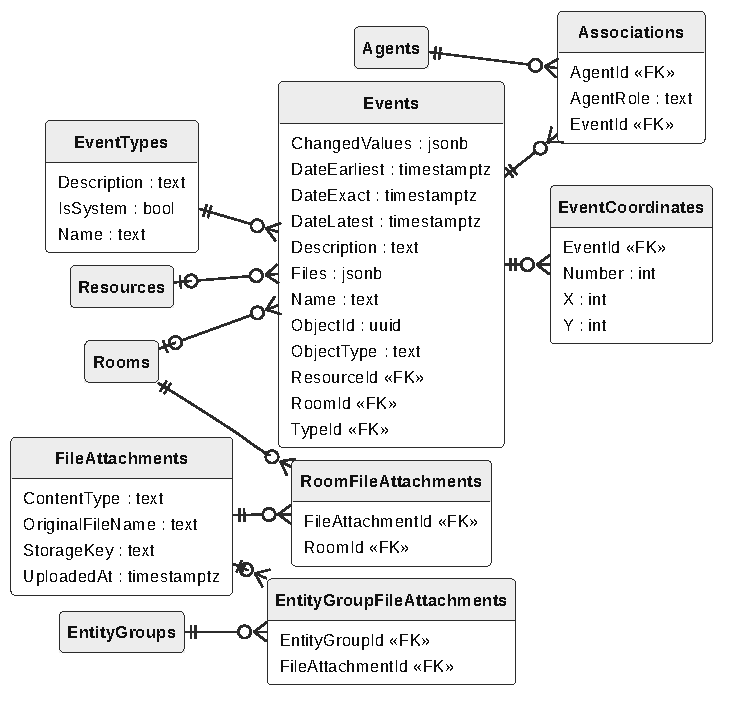
\includegraphics[width=12.5cm,height=0.86\textheight,keepaspectratio]{pics/er-history-files.pdf}
	\caption{Database schema, part 3: events, associations and file attachments.}
	\label{fig:er-history}
\end{figure}

